\documentclass{standalone}
\usepackage{tikz}
\begin{document}

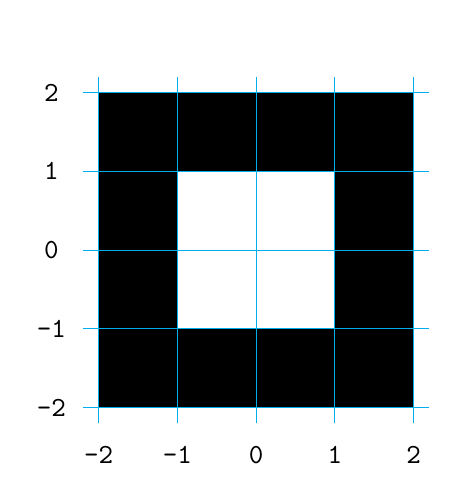
\begin{tikzpicture}
	\fill (-2,-2) rectangle (-1,2);
	\fill (-2,-2) rectangle (2,-1);
	\fill (1,-2) rectangle (2,2);
	\fill (-2,1) rectangle (2,2);
	\newcommand\overhang{0.2};
	\draw[cyan] (-2-\overhang, -2) -- (2+\overhang, -2);
	\draw[cyan] (-2-\overhang, -1) -- (2+\overhang, -1);
	\draw[cyan] (-2-\overhang, 0) -- (2+\overhang, 0);
	\draw[cyan] (-2-\overhang, 1) -- (2+\overhang, 1);
	\draw[cyan] (-2-\overhang, 2) -- (2+\overhang, 2);
	\draw[cyan] (-2, -2-\overhang) -- (-2, 2+\overhang);
	\draw[cyan] (-1, -2-\overhang) -- (-1, 2+\overhang);
	\draw[cyan] (0, -2-\overhang) -- (0, 2+\overhang);
	\draw[cyan] (1, -2-\overhang) -- (1, 2+\overhang);
	\draw[cyan] (2, -2-\overhang) -- (2, 2+\overhang);
	\foreach \i in {-2,...,2} {
		\draw (\i,-2.6) node {\texttt{\i}};
	}
	\foreach \i in {-2,...,2} {
		\draw (-2.6,\i) node {\texttt{\i}};
	}
	\draw[white] (0,2.6) node {\texttt{-012}};
\end{tikzpicture}

\end{document}
